\section{Introduction}

\paragraph{}
Massive scale datasets are becoming increasingly common today. Growth of 
the number of users who are actively using digital devices connected to the 
internet have vastly affected this phenomenon. Also there lies an interest 
in researchers to solve the problems which involves large datasets. Most of 
these datasets could be mapped to graphs to extract useful information, 
giving rise to the need of processing massive scale graphs. There are many 
practical scenarios where massive scale graphs are applied such as social 
networks, network traffic data and road networks.

\paragraph{}
It is much easier to work with graphs when they are static and small. However 
most of the natural graphs that are being encountered in the real world are 
dynamic. It becomes increasingly complex to handle the graph as the velocity
with which its edges gets updated increases. Large scale dynamic natural 
graphs are used by many companies today. Google uses PageRank 
algorithm\cite{brin_anatomy_1998} to map the links between the web pages. 
And facebook has a massive graph depicting the connections of each user 
on the platform. 

\paragraph{}
With the size of the massive scale graphs, it is difficult to evaluate the 
properties of them even after partitioning into multiple nodes. The graphs 
have to be summarized so that important information regarding the underlying 
dataset can be inferred easily.

\subsubsection{Motivation}
Being applied in a wide range of industrial and research applications, 
realtime property evaluation of streaming and dynamic natural graphs is a 
critical requirement in many scenarios. Graph summarization plays a big 
role in this as it reduces the computational resources required to evaluate 
the properties in a rather massive scale steaming graph. It would be beneficial 
for number of sectors in the process of summarizing streaming graphs were 
made efficient.

\subsection{Related work}

\subsubsection{Graph partitioning}
\paragraph{}
The size of modern datasets have become too large to be fit into a single 
machine. It has become unrealistic to try to process the graphs mapped to 
these massive datasets while keeping them in the memory of a single node. 
Hence there exist a need to partition those large scale graphs into multiple 
machines. However graph partitioning has been proved to be an NP-hard 
problem\cite{garey_simplified_1974}. Therefore the graph partitioning algorithms are only able to give 
sub-optimal solutions as of this date. Graph partitioning algorithms can be 
mainly divided into two, such that, Online Graph Partitioning Algorithms and 
Offline Graph Partitioning Algorithms. The offline partitioning algorithms 
such as METIS\cite{karypis_fast_1998}, Chaco\cite{hendrickson_chaco_1993}, 
SBV-cut\cite{kim_sbv-cut:_2012} need to load the entire graph into the 
memory for the algorithm to be run. But the online partitioning algorithms 
like PreferBig\cite{stanton_streaming_2012} and 
HoVerCut\cite{sajjad_boosting_2016} keeps a buffer of the edge streams and 
process them when the buffer gets full. 

\subsubsection{Graph summarization}

\begin{figure}[H]
    \centering
    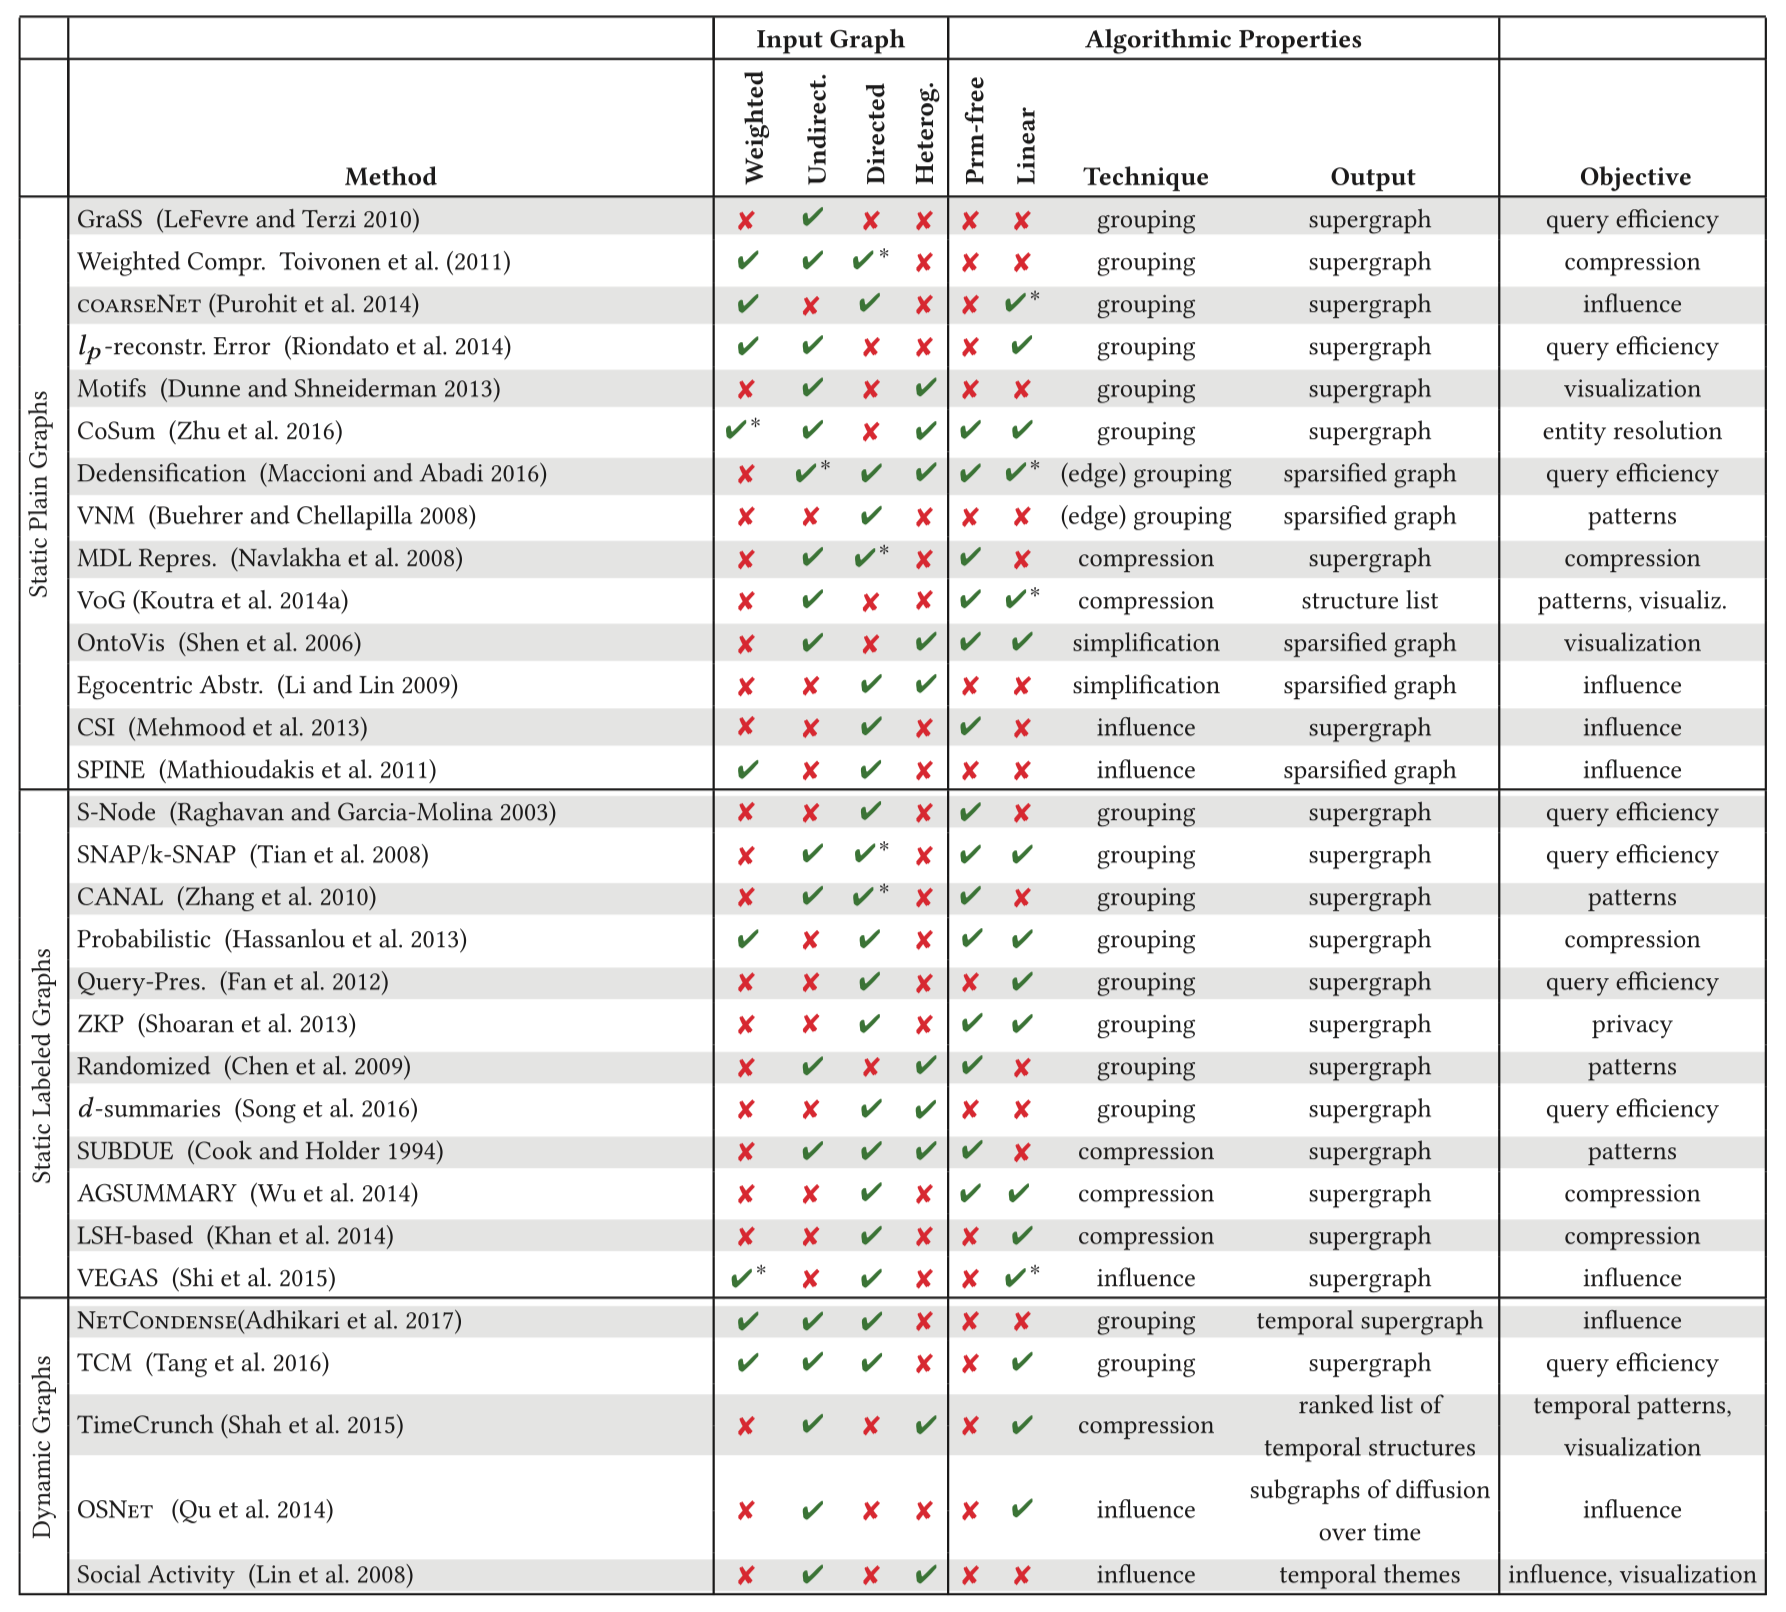
\includegraphics[width=\textwidth]{images/sum}
    \caption{Qualitative Comparison of All Graph Summarization Techniques Based on the Properties of the Input Graph\cite{liu_graph_2018}}
    % \label{fig:mesh1}
\end{figure}

\paragraph{}
There exist different techniques to summarize 
various types of graphs, i.e, static, dynamic, heterogeneous, streaming and 
domain dependant graphs. Summarizing each of these graphs prove to be a unique 
challenge while the objectives of summarization vary as well. Graph summarization 
is always a tradeoff between accuracy, efficiency and space. 

\paragraph{}
Some methods have already been devised to summarize the graph streams such 
as gSketch\cite{zhao_gsketch:_2011}, 
GMatrix\cite{khan_query-friendly_2016} and TCM\cite{tang_graph_2016}. 
These techniques permit only some types of queries 
to be run against the summaries with varying degrees of accuracies. This 
research aims to further analyze the properties of streaming graphs through 
summarization.

% \subsection{Research gap}

